\subsubsection{معماری \lr{Component-Based}}
\label{archCompBasedSec}
\begin{RTL}
در \lr{UML}،
یک \lr{Component} یک اثر زمان اجرا و یک واحد قابل
جایگزینی اساسی در نرم‌افزار است
که مشابه یک شیء بزرگ‌مقیاس شامل اشیاء کوچکتری است که واسط آن را
پیاده‌سازی می‌کنند. \lr{Component}ها دارای کپسوله‌سازی قوی و
واسط‌های مستقل از زبان برنامه‌نویسی و کاملاً تعریف شده هستند.
سیستم‌های مبتنی بر \lr{Component}
که از این اشیاء بزرگ‌مقیاس به عنوان واحدهای معماری استفاده می‌کنند، از نگهداری
آسان، جداسازی عیوب، استقلال از زبان منبع، سادگی توسعه و قابلیت استفاده مجدد
بهره‌مند می‌شوند. \lr{Component}ها معمولاً اشیاء کوچکتری را
برای هدف رفتاری مشترک در زمان اجرا جمع می‌کنند.
آنها دارای واسط‌های مبهم هستند، به این معنا که جزئیات
داخلی آنها از کلاینت مخفی است که این امر جایگزینی را تضمین می‌کند
اما ممکن است منجر به ناکارآمدی شود.
الگوی معماری مبتنی بر \lr{Component} \cite{ref4} معماری
سیستم را قوی و قابل استفاده مجدد می‌سازد اما ممکن است به دلیل
استفاده از کل \lr{Component}ها حتی اگر فقط بخشی از عملکرد آنها
استفاده شود، منابع اضافی مصرف کند.
\end{RTL}
\begin{figure}[h!]
\centering
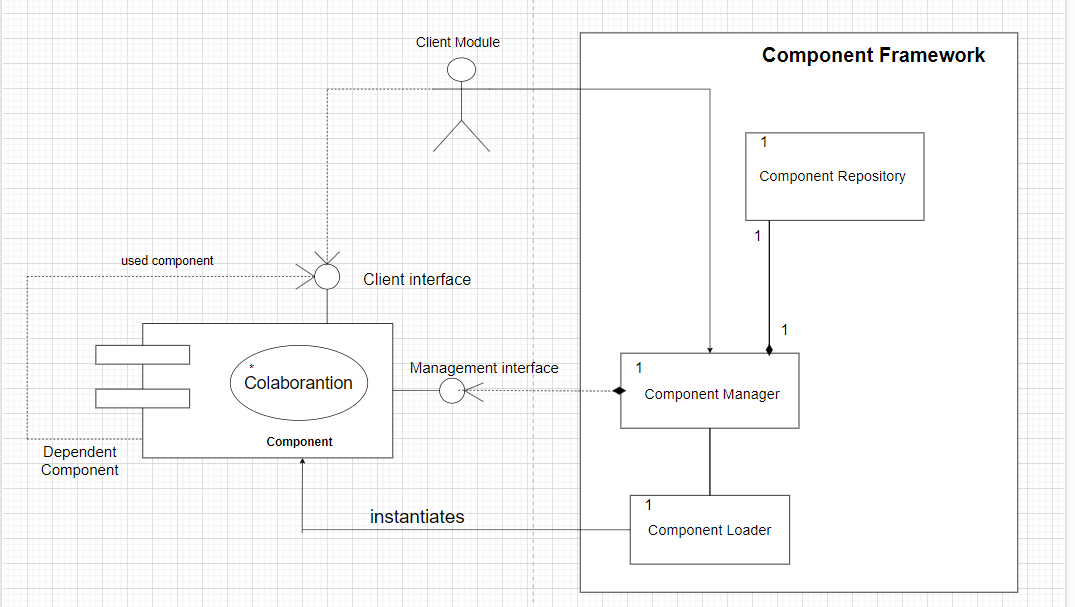
\includegraphics[scale=0.5]{images/first/component.png}
\caption{ساختار الگوی \lr{Component-Based}}
\end{figure}